
\subsection{LM-band imaging recipes}
\label{ssec:recipes_img_lm}
%------------------------------------------------------------------------------------------------------------------
\subsubsection{\REC*{metis_lm_img_flat}:  Flatfielding}
\label{lm_img_flatfield}
\label{rec:lm_img_flatfield}
\label{sssec:lm_img_flatfield}
\label{metis_lm_img_flat}
\label{rec:metis_lm_img_flat}
\label{sssec:metis_lm_img_flat}

The purpose of the flat-field calibration is to determine
pixel-to-pixel gain variations and large scale illumination variations
(due to inhomogeneities of optical elements in the telescope or
instrument). Calibration frames are obtained either during day time
using the black-body lamp of the \ac{WCU} (internal flats) or by taken
images of the twilight sky (twilight flats). Advantages and
disadvantages of the two types of flat are discussed in
\cite{METIS-calibration_plan}. Since the operational concept for
twilight flats needs to be refined during commissioning at the
telescope, the current recipe design is primarily valid for internal
flats.

This recipe creates a master flat for the HAWAII2RG detector (LM-band
imaging) from lamp or sky images matched by various setup parameters
as detailed below.  A set of internal flats includes a number of
exposures with \CODE{LAMP OFF}, which will be used for dark
subtraction. For twilight flats a master dark will be subtracted. The
master flat is obtained by the slope of a linear fit of the pixel
values against the illumination level of the exposures.

The quality control parameters give various statistics for each input
frame (mean, standard deviation, etc.), the standard deviation of the
normalised master flat and the number of bad pixels identified by the
recipe. If a bad-pixel map is provided on input, it is updated,
otherwise a new one is created.

\begin{recipedef}
  Name:                & \REC{metis_lm_img_flat} \\
  Purpose:             & Create master flat for L/M band detectors \\
%  Requirements:        & \REQ{METIS-XXXX} \\
%  Type:                & Calibration | Science | Technical \\
%  Templates:           & \TPL{...} \\
  Primary input:       & \RAW{LM_FLAT_LAMP_RAW} or \RAW{LM_FLAT_TWILIGHT_RAW} (N$\times$) \\
  Secondary inputs:    & \PROD{BADPIX_MAP_2RG} (optional) \\
                       & \hyperref[dataitem:gain_map_det]{\STATCALIB*{GAIN_MAP_2RG}} \\
                       & \hyperref[dataitem:linearity_det]{\PROD*{LINEARITY_2RG}} \\
                       & \PROD{MASTER_DARK_2RG} \\
                       & \EXTCALIB{PERSISTENCE_MAP} (optional) \\
  Matched keywords:    & \FITS{DET.DIT} \\
                       & \FITS{DET.NDIT} \\
                       & \FITS{DRS.FILTER} \\
  Parameters:          & \CODE{metis_lm_img_flat.stacking.method}: string\newline Name of the method used to combine the input images (\underline{\texttt{average}}, \texttt{median}) \\
                       & \CODE{metis_lm_img_flat.outliers.kappa_low}: int\newline Lower threshold for bad pixels, default \texttt{10} \\
                       & \CODE{metis_lm_img_flat.outliers.kappa_high}: int\newline Upper threshold for bad pixels, default \texttt{10} \\
  Algorithm:           & For internal flats: call \REC{metis_det_dark} with LAMP OFF images to create dark frame. \\
                       & Subtract internal dark or master dark from flat exposures. \\
                       & Call \REC{metis_lm_img_flat} to fit slope of pixel values against illumination level. \\
                       & Frames with the same exposure time will be averaged. \\
                       & Compute median or average of input frames to improve statistics. \\
                       & Call \texttt{metis\_update\_lm\_flat\_mask} to flag deviant pixels. \\
  Output data:         & \PROD{BADPIX_MAP_2RG} \\
                       & \PROD{MASTER_IMG_FLAT_LAMP_LM} or \PROD{MASTER_IMG_FLAT_TWILIGHT_LM} \\
%  Expected accuracies: & \\
  QC1 parameters:      & \QC{QC LM FLAT MEAN} \\
                       & \QC{QC LM FLAT MEDIAN MAX} \\
                       & \QC{QC LM FLAT MEDIAN MIN} \\
                       & \QC{QC LM FLAT MEDIAN RMS} \\
                       & \QC{QC LM FLAT RMS} \\
                       & \QC{QC LM MFLAT NBADPIX} \\
                       & \QC{QC LM MFLAT RMS} \\
\end{recipedef}



\begin{figure}[hb]
  \centering
    \def \globalscale {0.700000}
    \fontsize{10}{12}\selectfont
    %% Flowchart of metis_lm_img_flat, generated by metisp/drld/generate_drld.py -- do not edit

% ADDING NEW DEFINITIONS -------------------------------------------- start
\definecolor{listingbg}{gray}{0.95}
\definecolor{darkgreen}{rgb}{0.0, 0.7, 0.0}
\definecolor{darkblue} {rgb}{0.0, 0.0, 0.7}
\definecolor{cyan} {rgb}{0.0, 0.4, 0.4}
\definecolor{darkred}  {rgb}{0.7, 0.0, 0.0}
\definecolor{darkorange}{rgb}{1.0, 0.49, 0.0}
\definecolor{violet}{rgb}{255, 0, 255}
\definecolor{turq}{rgb}{0.0, 0.7, 0.8}
\definecolor{fits}{rgb}{0.4, 0.1, 1}


\makeatletter
\lstdefinestyle{RAWstyle}{%
  basicstyle=\ttfamily\color{black}%
  \lst@ifdisplaystyle\scriptsize\fi}

\lstdefinestyle{PARstyle}{%
  basicstyle=\ttfamily\color{black}%
  \lst@ifdisplaystyle\scriptsize\fi}

\lstdefinestyle{DRLstyle}{%
  basicstyle=\ttfamily\color{black}%
  \lst@ifdisplaystyle\scriptsize\fi}

\lstdefinestyle{RECstyle}{%
  basicstyle=\ttfamily\color{black}%
  \lst@ifdisplaystyle\scriptsize\fi}

\lstdefinestyle{QCstyle}{%
  basicstyle=\ttfamily\color{black}%
  \lst@ifdisplaystyle\scriptsize\fi}

\lstdefinestyle{TPLstyle}{%
  basicstyle=\ttfamily\color{black}%
  \lst@ifdisplaystyle\scriptsize\fi}

\lstdefinestyle{PRODstyle}{%
  basicstyle=\ttfamily\color{black}%
  \lst@ifdisplaystyle\scriptsize\fi}

\lstdefinestyle{EXTCALIBstyle}{%
  basicstyle=\ttfamily\color{black}%
  \lst@ifdisplaystyle\scriptsize\fi}

\lstdefinestyle{STATCALIBstyle}{%
  basicstyle=\ttfamily\color{black}%
  \lst@ifdisplaystyle\scriptsize\fi}

\lstdefinestyle{FITSstyle}{%
  basicstyle=\ttfamily\color{black}%
  \lst@ifdisplaystyle\scriptsize\fi}
\makeatother

\input{recipe_config}
%% The picture is set in a box and only scaled down when it would not fit the page.
\ifdefined\flowchartbox\else\newsavebox{\flowchartbox}\fi
\sbox{\flowchartbox}{%
\begin{tikzpicture}
  [x=1cm,
  y=-1cm,
  align=center,
  node distance=2cm and 3.5cm,
  redstep/.append style={minimum height=0.8cm, text width=3.8cm}]
  \sffamily
  \pic (start){start};
  \node (input) [below=0.75cm of start-m, input] {%
    N$\times$ \RAW{LM_FLAT_LAMP_RAW} \\[-0.5ex] {\footnotesize or} \\[-0.5ex] N$\times$ \RAW{LM_FLAT_TWILIGHT_RAW}};

  %% algorithm steps
  \node (step_detectorsignatureremoval) [below=5.6cm of input, redstep]{%
    detector signature removal};
  \node (step_linearfitslope) [below=0.6cm of step_detectorsignatureremoval, redstep]{%
    linear fit (slope)};
  \pic (stop) [below=3.16cm of step_linearfitslope] {stop};

  \draw [connection_arrow] (start-m) -- (input);
  \draw [connection_arrow] (input) -- (step_detectorsignatureremoval);
  \draw [connection_arrow] (step_detectorsignatureremoval) -- (step_linearfitslope);
  \draw [connection_arrow] (step_linearfitslope) -- (stop-t);

  %% calibration inputs, attached above the step that consumes them
  \node (connect_badpixmap) [connection] at ($(input.south) + (0, 0.97)$) {};
  \node (badpixmap) [left=of connect_badpixmap, calproduct] {\PROD{BADPIX_MAP_2RG}};
  \draw [connection_arrow, dashed] (badpixmap) -- (connect_badpixmap);
  \node (connect_gainmap) [connection] at ($(input.south) + (0, 1.98)$) {};
  \node (gainmap) [left=of connect_gainmap, external] {\hyperref[dataitem:gain_map_det]{\STATCALIB*{GAIN_MAP_2RG}}};
  \draw [connection_arrow] (gainmap) -- (connect_gainmap);
  \node (connect_linearity) [connection] at ($(input.south) + (0, 2.98)$) {};
  \node (linearity) [left=of connect_linearity, calproduct] {\hyperref[dataitem:linearity_det]{\PROD*{LINEARITY_2RG}}};
  \draw [connection_arrow] (linearity) -- (connect_linearity);
  \node (connect_masterdark) [connection] at ($(input.south) + (0, 3.98)$) {};
  \node (masterdark) [left=of connect_masterdark, calproduct] {\PROD{MASTER_DARK_2RG}};
  \draw [connection_arrow] (masterdark) -- (connect_masterdark);
  \node (connect_persistencemap) [connection] at ($(input.south) + (0, 4.97)$) {};
  \node (persistencemap) [left=of connect_persistencemap, external] {\EXTCALIB{PERSISTENCE_MAP}};
  \draw [connection_arrow, dashed] (persistencemap) -- (connect_persistencemap);

  %% products, attached below the step that produces them
  \node (connect_badpixmap) [connection] at ($(step_linearfitslope.south) + (0, 0.62)$) {};
  \node (badpixmap) [right=of connect_badpixmap, calproduct] {\PROD{BADPIX_MAP_2RG}};
  \draw [connection_arrow] (connect_badpixmap) -- (badpixmap);
  \node (connect_masterflat) [connection] at ($(step_linearfitslope.south) + (0, 1.98)$) {};
  \node (masterflat) [right=of connect_masterflat, calproduct] {\PROD{MASTER_IMG_FLAT_LAMP_LM} \\[-0.5ex] {\footnotesize or} \\[-0.5ex] \PROD{MASTER_IMG_FLAT_TWILIGHT_LM}};
  \draw [connection_arrow] (connect_masterflat) -- (masterflat);

  \draw [frame] ($(input.south) + (-2.85, 0.12)$) rectangle
  ($(step_linearfitslope.south) + (2.85, 2.7600000000000002)$);
  \node [framecolor, anchor=north west] at ($(input.south) + (-2.85, 0.12)$) {%
    \REC{metis_lm_img_flat}};
\end{tikzpicture}}%
\ifdim\ht\flowchartbox>\dimexpr\textheight-4\baselineskip\relax
  \resizebox{!}{\dimexpr\textheight-4\baselineskip\relax}{\usebox{\flowchartbox}}%
\else\ifdim\wd\flowchartbox>\linewidth
  \resizebox{\linewidth}{!}{\usebox{\flowchartbox}}%
\else
  \usebox{\flowchartbox}%
\fi\fi

% ADDING NEW DEFINITIONS -------------------------------------------- start
\definecolor{listingbg}{gray}{0.95}
\definecolor{darkgreen}{rgb}{0.0, 0.7, 0.0}
\definecolor{darkblue} {rgb}{0.0, 0.0, 0.7}
\definecolor{cyan} {rgb}{0.0, 0.4, 0.4}
\definecolor{darkred}  {rgb}{0.7, 0.0, 0.0}
\definecolor{darkorange}{rgb}{1.0, 0.49, 0.0}
\definecolor{violet}{rgb}{255, 0, 255}
\definecolor{turq}{rgb}{0.0, 0.7, 0.8}
\definecolor{fits}{rgb}{0.4, 0.1, 1}


\makeatletter
\lstdefinestyle{RAWstyle}{%
  basicstyle=\ttfamily\color{fits}%
  \lst@ifdisplaystyle\scriptsize\fi}

\lstdefinestyle{PARstyle}{%
  basicstyle=\ttfamily\color{cyan}%
  \lst@ifdisplaystyle\scriptsize\fi}

\lstdefinestyle{DRLstyle}{%
  basicstyle=\ttfamily\color{violet}%
  \lst@ifdisplaystyle\scriptsize\fi}

\lstdefinestyle{RECstyle}{%
  basicstyle=\ttfamily\color{darkgreen}%
  \lst@ifdisplaystyle\scriptsize\fi}

%% Write QC parameters like this: \QC{QC_SOMETHING_OR_OTHER}
\lstdefinestyle{QCstyle}{%
  basicstyle=\ttfamily\color{darkblue}%
  \lst@ifdisplaystyle\scriptsize\fi}

%% Write templates like this: \TPL{DARK_LM}
\lstdefinestyle{TPLstyle}{%
  basicstyle=\ttfamily\color{darkred}%
  \lst@ifdisplaystyle\scriptsize\fi}

%% Write products like this: \PROD{SOME_THING}
\lstdefinestyle{PRODstyle}{%
  basicstyle=\ttfamily\color{darkorange}%
  \lst@ifdisplaystyle\scriptsize\fi}

%% external calib files
\lstdefinestyle{EXTCALIBstyle}{%
  basicstyle=\ttfamily\color{Turquoise}%
  \lst@ifdisplaystyle\scriptsize\fi}

% static calib files
\lstdefinestyle{STATCALIBstyle}{%
  basicstyle=\ttfamily\color{teal}%
  \lst@ifdisplaystyle\scriptsize\fi}

% static calib files
\lstdefinestyle{FITSstyle}{%
  basicstyle=\ttfamily\color{black}%
  \lst@ifdisplaystyle\scriptsize\fi}
\makeatother


  \caption[Recipe: \REC*{metis_lm_img_flat}]{\REC*{metis_lm_img_flat} --
    creation of \CODE{IMG_LM} master flatfield.}
  \label{fig:metis_lm_img_flat}
\end{figure}
%    \TODO{Include averaging of frames at same illumination in figure}

%------------------------------------------------------------------------------------------------------------------
\clearpage
\subsubsection{\REC*{metis_lm_img_basic_reduce}:  Basic reduction}
\label{lm_img_basic}
\label{rec:lm_img_basic}
\label{sssec:lm_img_basic}
\label{metis_lm_img_basic_reduce}
\label{rec:metis_lm_img_basic_reduce}
\label{sssec:metis_lm_img_basic_reduce}

%\TODO{New recipe -- this may be too basic and could be joined with the background subtraction.}

This recipe performs the basic reduction of raw exposures from the
LM-band imager, i.e.\ dark subtraction, flat fielding and removing
other instrumental signals. It is used for both standard and science exposures.

This recipe analyses the masked detector regions for channel offset correction, crosstalk (Section~\ref{ssec:criticaldetetctormasks}) and removal of detector artefacts (electronic ghosts).
In the horizontal dimension, the masked pixels are used to correct for each channel offset.
In the vertical dimension, the masked pixels are used to correct for cross-talk.
% From Rof https://polarion.astron.nl/polarion/#/project/METIS/workitem?id=METIS-6089
% I am not sure whether the masked region should be removed from pipeline products (at least not as in this very general statement). For some products, it can be useful to inspect the masked regions and that would be much more cumbersome if they were removed from products that have undergone any form or processing. I would remove the last sentence from the requirement, or at least rephrase it. For some or even most of the high-level products, the masked region would be a nuisance if present so for most pipeline products one would indeed like to have it removed

Basic statistics of the images can be used to screen for saturation.

\begin{recipedef}
  Name:                & \REC{metis_lm_img_basic_reduce} \\
  Purpose:             & Basic science image data processing \\
%  Requirements:        & \REQ{METIS-XXXX} \\
%  Type:                & Calibration | Science | Technical \\
%  Templates:           & \TPL{...} \\
  Primary input:       & \RAW{LM_IMAGE_SCI_RAW} or \RAW{LM_IMAGE_SKY_RAW} or \RAW{LM_IMAGE_STD_RAW} (N$\times$) \\
  Secondary inputs:    & \PROD{BADPIX_MAP_2RG} (optional) \\
                       & \hyperref[dataitem:gain_map_det]{\STATCALIB*{GAIN_MAP_2RG}} \\
                       & \hyperref[dataitem:linearity_det]{\PROD*{LINEARITY_2RG}} \\
                       & \PROD{MASTER_DARK_2RG} \\
                       & \PROD{MASTER_IMG_FLAT_LAMP_LM} or \PROD{MASTER_IMG_FLAT_TWILIGHT_LM} \\
                       & \EXTCALIB{PERSISTENCE_MAP} (optional) \\
  Matched keywords:    & \FITS{DET.DIT} \\
                       & \FITS{DET.NDIT} \\
                       & \FITS{DRS.FILTER} \\
  Parameters:          & \CODE{metis_lm_img_basic_reduce.stacking.method}\newline Name of the method used to combine the input images (\texttt{add}, \texttt{average}, \texttt{median}), default \texttt{add} \\
  Algorithm:           & Remove crosstalk, correct non-linearity \\
                       & Analyse and optionally remove masked regions \\
                       & Subtract dark, divide by flat \\
                       & Remove blank sky pattern \\
  Output data:         & \PROD{LM_SCI_BASIC_REDUCED} or \PROD{LM_SKY_BASIC_REDUCED} or \PROD{LM_STD_BASIC_REDUCED} \\
%  Expected accuracies: & \\
  QC1 parameters:      & \QC{QC LM IMG MEDIAN} \\
                       & \QC{QC LM IMG PEAK} \\
                       & \QC{QC LM IMG STANDARD DEVIATION} \\
\end{recipedef}



\newgeometry{bottom=0.1cm, right=0.1cm, left=0.1cm, top=0.1cm}
\begin{figure}[hb]
  \centering
    \def \globalscale {0.700000}
    \fontsize{10}{12}\selectfont
    %% Flowchart of metis_lm_img_basic_reduce, generated by metisp/drld/generate_drld.py -- do not edit

% ADDING NEW DEFINITIONS -------------------------------------------- start
\definecolor{listingbg}{gray}{0.95}
\definecolor{darkgreen}{rgb}{0.0, 0.7, 0.0}
\definecolor{darkblue} {rgb}{0.0, 0.0, 0.7}
\definecolor{cyan} {rgb}{0.0, 0.4, 0.4}
\definecolor{darkred}  {rgb}{0.7, 0.0, 0.0}
\definecolor{darkorange}{rgb}{1.0, 0.49, 0.0}
\definecolor{violet}{rgb}{255, 0, 255}
\definecolor{turq}{rgb}{0.0, 0.7, 0.8}
\definecolor{fits}{rgb}{0.4, 0.1, 1}


\makeatletter
\lstdefinestyle{RAWstyle}{%
  basicstyle=\ttfamily\color{black}%
  \lst@ifdisplaystyle\scriptsize\fi}

\lstdefinestyle{PARstyle}{%
  basicstyle=\ttfamily\color{black}%
  \lst@ifdisplaystyle\scriptsize\fi}

\lstdefinestyle{DRLstyle}{%
  basicstyle=\ttfamily\color{black}%
  \lst@ifdisplaystyle\scriptsize\fi}

\lstdefinestyle{RECstyle}{%
  basicstyle=\ttfamily\color{black}%
  \lst@ifdisplaystyle\scriptsize\fi}

\lstdefinestyle{QCstyle}{%
  basicstyle=\ttfamily\color{black}%
  \lst@ifdisplaystyle\scriptsize\fi}

\lstdefinestyle{TPLstyle}{%
  basicstyle=\ttfamily\color{black}%
  \lst@ifdisplaystyle\scriptsize\fi}

\lstdefinestyle{PRODstyle}{%
  basicstyle=\ttfamily\color{black}%
  \lst@ifdisplaystyle\scriptsize\fi}

\lstdefinestyle{EXTCALIBstyle}{%
  basicstyle=\ttfamily\color{black}%
  \lst@ifdisplaystyle\scriptsize\fi}

\lstdefinestyle{STATCALIBstyle}{%
  basicstyle=\ttfamily\color{black}%
  \lst@ifdisplaystyle\scriptsize\fi}

\lstdefinestyle{FITSstyle}{%
  basicstyle=\ttfamily\color{black}%
  \lst@ifdisplaystyle\scriptsize\fi}
\makeatother

\input{recipe_config}
%% The picture is set in a box and only scaled down when it would not fit the page.
\ifdefined\flowchartbox\else\newsavebox{\flowchartbox}\fi
\sbox{\flowchartbox}{%
\begin{tikzpicture}
  [x=1cm,
  y=-1cm,
  align=center,
  node distance=2cm and 3.5cm,
  redstep/.append style={minimum height=0.8cm, text width=3.8cm}]
  \sffamily
  \pic (start){start};
  \node (input) [below=0.75cm of start-m, input] {%
    \textsl{N} \RAW{LM_IMAGE_SCI_RAW} \\[-0.5ex] {\footnotesize or} \\[-0.5ex] \textsl{N} \RAW{LM_IMAGE_SKY_RAW} \\[-0.5ex] {\footnotesize or} \\[-0.5ex] \textsl{N} \RAW{LM_IMAGE_STD_RAW}};

  %% algorithm steps
  \node (step_correctnonlinearity) [below=3.6cm of input, redstep]{%
    Correct non-linearity};
  \node (step_correctpersistence) [below=1.25cm of step_correctnonlinearity, redstep]{%
    Correct persistence};
  \node (step_subtractdark) [below=1.25cm of step_correctpersistence, redstep]{%
    subtract dark};
  \node (step_dividebyflat) [below=1.96cm of step_subtractdark, redstep]{%
    divide by flat};
  \node (step_analyseandremovemaskedre) [below=0.6cm of step_dividebyflat, redstep]{%
    analyse and remove masked regions};
  \pic (stop) [below=2.89cm of step_analyseandremovemaskedre] {stop};

  \draw [connection_arrow] (start-m) -- (input);
  \draw [connection_arrow] (input) -- (step_correctnonlinearity);
  \draw [connection_arrow] (step_correctnonlinearity) -- (step_correctpersistence);
  \draw [connection_arrow] (step_correctpersistence) -- (step_subtractdark);
  \draw [connection_arrow] (step_subtractdark) -- (step_dividebyflat);
  \draw [connection_arrow] (step_dividebyflat) -- (step_analyseandremovemaskedre);
  \draw [connection_arrow] (step_analyseandremovemaskedre) -- (stop-t);

  %% calibration inputs, attached above the step that consumes them
  \node (connect_badpixmap) [connection] at ($(input.south) + (0, 0.97)$) {};
  \node (badpixmap) [left=of connect_badpixmap, calproduct] {\PROD{BADPIX_MAP_2RG}};
  \draw [connection_arrow, dashed] (badpixmap) -- (connect_badpixmap);
  \node (connect_gainmap) [connection] at ($(input.south) + (0, 1.98)$) {};
  \node (gainmap) [left=of connect_gainmap, external] {\hyperref[dataitem:gain_map_det]{\STATCALIB*{GAIN_MAP_2RG}}};
  \draw [connection_arrow] (gainmap) -- (connect_gainmap);
  \node (connect_linearity) [connection] at ($(input.south) + (0, 2.98)$) {};
  \node (linearity) [left=of connect_linearity, calproduct] {\hyperref[dataitem:linearity_det]{\PROD*{LINEARITY_2RG}}};
  \draw [connection_arrow] (linearity) -- (connect_linearity);
  \node (connect_persistencemap) [connection] at ($(step_correctnonlinearity.south) + (0, 0.62)$) {};
  \node (persistencemap) [left=of connect_persistencemap, external] {\EXTCALIB{PERSISTENCE_MAP}};
  \draw [connection_arrow, dashed] (persistencemap) -- (connect_persistencemap);
  \node (connect_masterdark) [connection] at ($(step_correctpersistence.south) + (0, 0.62)$) {};
  \node (masterdark) [left=of connect_masterdark, calproduct] {\PROD{MASTER_DARK_2RG}};
  \draw [connection_arrow] (masterdark) -- (connect_masterdark);
  \node (connect_masterflat) [connection] at ($(step_subtractdark.south) + (0, 0.98)$) {};
  \node (masterflat) [left=of connect_masterflat, calproduct] {\PROD{MASTER_IMG_FLAT_LAMP_LM} \\[-0.5ex] {\footnotesize or} \\[-0.5ex] \PROD{MASTER_IMG_FLAT_TWILIGHT_LM}};
  \draw [connection_arrow] (masterflat) -- (connect_masterflat);

  %% products, attached below the step that produces them
  \node (connect_basicreduced) [connection] at ($(step_analyseandremovemaskedre.south) + (0, 1.34)$) {};
  \node (basicreduced) [right=of connect_basicreduced, calproduct] {\PROD{LM_SCI_BASIC_REDUCED} \\[-0.5ex] {\footnotesize or} \\[-0.5ex] \PROD{LM_SKY_BASIC_REDUCED} \\[-0.5ex] {\footnotesize or} \\[-0.5ex] \PROD{LM_STD_BASIC_REDUCED}};
  \draw [connection_arrow] (connect_basicreduced) -- (basicreduced);

  \draw [frame] ($(input.south) + (-2.85, 0.12)$) rectangle
  ($(step_analyseandremovemaskedre.south) + (2.85, 2.49)$);
  \node [framecolor, anchor=north west] at ($(input.south) + (-2.85, 0.12)$) {%
    \REC{metis_lm_img_basic_reduce}};
\end{tikzpicture}}%
\ifdim\ht\flowchartbox>\dimexpr\textheight-4\baselineskip\relax
  \resizebox{!}{\dimexpr\textheight-4\baselineskip\relax}{\usebox{\flowchartbox}}%
\else\ifdim\wd\flowchartbox>\linewidth
  \resizebox{\linewidth}{!}{\usebox{\flowchartbox}}%
\else
  \usebox{\flowchartbox}%
\fi\fi

% ADDING NEW DEFINITIONS -------------------------------------------- start
\definecolor{listingbg}{gray}{0.95}
\definecolor{darkgreen}{rgb}{0.0, 0.7, 0.0}
\definecolor{darkblue} {rgb}{0.0, 0.0, 0.7}
\definecolor{cyan} {rgb}{0.0, 0.4, 0.4}
\definecolor{darkred}  {rgb}{0.7, 0.0, 0.0}
\definecolor{darkorange}{rgb}{1.0, 0.49, 0.0}
\definecolor{violet}{rgb}{255, 0, 255}
\definecolor{turq}{rgb}{0.0, 0.7, 0.8}
\definecolor{fits}{rgb}{0.4, 0.1, 1}


\makeatletter
\lstdefinestyle{RAWstyle}{%
  basicstyle=\ttfamily\color{fits}%
  \lst@ifdisplaystyle\scriptsize\fi}

\lstdefinestyle{PARstyle}{%
  basicstyle=\ttfamily\color{cyan}%
  \lst@ifdisplaystyle\scriptsize\fi}

\lstdefinestyle{DRLstyle}{%
  basicstyle=\ttfamily\color{violet}%
  \lst@ifdisplaystyle\scriptsize\fi}

\lstdefinestyle{RECstyle}{%
  basicstyle=\ttfamily\color{darkgreen}%
  \lst@ifdisplaystyle\scriptsize\fi}

%% Write QC parameters like this: \QC{QC_SOMETHING_OR_OTHER}
\lstdefinestyle{QCstyle}{%
  basicstyle=\ttfamily\color{darkblue}%
  \lst@ifdisplaystyle\scriptsize\fi}

%% Write templates like this: \TPL{DARK_LM}
\lstdefinestyle{TPLstyle}{%
  basicstyle=\ttfamily\color{darkred}%
  \lst@ifdisplaystyle\scriptsize\fi}

%% Write products like this: \PROD{SOME_THING}
\lstdefinestyle{PRODstyle}{%
  basicstyle=\ttfamily\color{darkorange}%
  \lst@ifdisplaystyle\scriptsize\fi}

%% external calib files
\lstdefinestyle{EXTCALIBstyle}{%
  basicstyle=\ttfamily\color{Turquoise}%
  \lst@ifdisplaystyle\scriptsize\fi}

% static calib files
\lstdefinestyle{STATCALIBstyle}{%
  basicstyle=\ttfamily\color{teal}%
  \lst@ifdisplaystyle\scriptsize\fi}

% static calib files
\lstdefinestyle{FITSstyle}{%
  basicstyle=\ttfamily\color{black}%
  \lst@ifdisplaystyle\scriptsize\fi}
\makeatother


  \caption[Recipe: \REC*{metis_lm_img_basic_reduce}]{\REC*{metis_lm_img_basic_reduce} --
    basic reduction of \CODE{IMG_LM} data.}
  \label{fig:metis_lm_img_basic_reduce}
\end{figure}
\restoregeometry

%------------------------------------------------------------------------------------------------------------------
\clearpage
\subsubsection{\REC*{metis_lm_img_background}: Background subtraction}
\label{lm_img_background}
\label{rec:lm_img_background}
\label{sssec:lm_img_background}
\label{metis_lm_img_background}
\label{rec:metis_lm_img_background}
\label{sssec:metis_lm_img_background}

This recipe estimates and subtracts the background from LM-band
imaging data. Thermal background emission from the atmosphere,
telescope and warm parts of the instrument dominate the photon count
in mid-infrared observations. Accurate determination and removal of
background counts is therefore crucial to make MIR data scientifically
usable.

A set of observations will consist of a number of exposures
of the field, where the offsets are achieved by either using the internal
chopper of METIS or by telescope nodding. For extended objects, the
telescope will be used to perform ``out-of-field nodding'', i.e.\
observe nearby blank patches of sky interlaced with the target
observations. Imaging observations are performed in pupil-tracking
mode, hence angular offsetting of the field is automatic.

For in-field-offset exposures, all offset exposures will be
averaged to obtain the background estimate. In order to only average
the background contribution, an iterative procedure of object
detection and masking will be employed. Averaging will be done using a
robust estimator of the mean (e.g.\ median).

For extended objects, all out-of-field exposures will be averaged
(with object rejection) and subtracted off the in-field exposures.

For more information see Section~\ref{sssec:lmbandsbackgroundsubtracion}.

% Moved to https://github.com/AstarVienna/METIS_DRLD/issues/99
% \TODO{Object catalogues of the target exposures could be created within this
% recipe or in a separate recipe. The catalogue should contain for each
% object: pixel coordinates ($x$, $y$), world coordinates ($\alpha$,
% $\delta$) based on telescope pointing and derotator information, total
% counts within an aperture.}
%
% \TODO{Is this good enough for HCI images or do we need more?}

\begin{recipedef}
  Name:                & \REC{metis_lm_img_background} \\
  Purpose:             & Basic reduction of raw exposures from the \{band\} imager \\
%  Requirements:        & \REQ{METIS-XXXX} \\
%  Type:                & Calibration | Science | Technical \\
%  Templates:           & \TPL{...} \\
  Primary input:       & \PROD{LM_SCI_BASIC_REDUCED} or \PROD{LM_SKY_BASIC_REDUCED} or \PROD{LM_STD_BASIC_REDUCED} \\
  Secondary inputs:    & \PROD{LM_SKY_BASIC_REDUCED} \\
  Matched keywords:    & \FITS{DRS.FILTER} \\
  Parameters:          & \CODE{metis_lm_img_background.stacking.method}\newline Name of the method used to combine the input images (\texttt{add}, \texttt{average}, \texttt{median}), default \texttt{add} \\
  Algorithm:           & Average all or SKY exposures with object rejection \\
                       & Subtract background \\
  Output data:         & \PROD{LM_SCI_BKG} or \PROD{LM_STD_BKG} \\
                       & \PROD{LM_SCI_BKG_SUBTRACTED} or \PROD{LM_STD_BKG_SUBTRACTED} \\
                       & \PROD{LM_SCI_OBJECT_CAT} or \PROD{LM_STD_OBJECT_CAT} \\
%  Expected accuracies: & \\
  QC1 parameters:      & \QC{QC LM IMG BKG MEDIAN} \\
                       & \QC{QC LM IMG BKG MEDIAN DEVIATION} \\
\end{recipedef}



\begin{figure}[hb]
    \centering
    \def \globalscale {0.700000}
    \fontsize{10}{12}\selectfont
    %% Flowchart of metis_lm_img_background, generated by metisp/drld/generate_drld.py -- do not edit

% ADDING NEW DEFINITIONS -------------------------------------------- start
\definecolor{listingbg}{gray}{0.95}
\definecolor{darkgreen}{rgb}{0.0, 0.7, 0.0}
\definecolor{darkblue} {rgb}{0.0, 0.0, 0.7}
\definecolor{cyan} {rgb}{0.0, 0.4, 0.4}
\definecolor{darkred}  {rgb}{0.7, 0.0, 0.0}
\definecolor{darkorange}{rgb}{1.0, 0.49, 0.0}
\definecolor{violet}{rgb}{255, 0, 255}
\definecolor{turq}{rgb}{0.0, 0.7, 0.8}
\definecolor{fits}{rgb}{0.4, 0.1, 1}


\makeatletter
\lstdefinestyle{RAWstyle}{%
  basicstyle=\ttfamily\color{black}%
  \lst@ifdisplaystyle\scriptsize\fi}

\lstdefinestyle{PARstyle}{%
  basicstyle=\ttfamily\color{black}%
  \lst@ifdisplaystyle\scriptsize\fi}

\lstdefinestyle{DRLstyle}{%
  basicstyle=\ttfamily\color{black}%
  \lst@ifdisplaystyle\scriptsize\fi}

\lstdefinestyle{RECstyle}{%
  basicstyle=\ttfamily\color{black}%
  \lst@ifdisplaystyle\scriptsize\fi}

\lstdefinestyle{QCstyle}{%
  basicstyle=\ttfamily\color{black}%
  \lst@ifdisplaystyle\scriptsize\fi}

\lstdefinestyle{TPLstyle}{%
  basicstyle=\ttfamily\color{black}%
  \lst@ifdisplaystyle\scriptsize\fi}

\lstdefinestyle{PRODstyle}{%
  basicstyle=\ttfamily\color{black}%
  \lst@ifdisplaystyle\scriptsize\fi}

\lstdefinestyle{EXTCALIBstyle}{%
  basicstyle=\ttfamily\color{black}%
  \lst@ifdisplaystyle\scriptsize\fi}

\lstdefinestyle{STATCALIBstyle}{%
  basicstyle=\ttfamily\color{black}%
  \lst@ifdisplaystyle\scriptsize\fi}

\lstdefinestyle{FITSstyle}{%
  basicstyle=\ttfamily\color{black}%
  \lst@ifdisplaystyle\scriptsize\fi}
\makeatother

\input{recipe_config}
%% The picture is set in a box and only scaled down when it would not fit the page.
\ifdefined\flowchartbox\else\newsavebox{\flowchartbox}\fi
\sbox{\flowchartbox}{%
\begin{tikzpicture}
  [x=1cm,
  y=-1cm,
  align=center,
  node distance=2cm and 3.5cm,
  redstep/.append style={minimum height=0.8cm, text width=3.8cm}]
  \sffamily
  \pic (start){start};
  \node (input) [below=0.75cm of start-m, input] {%
    \PROD{LM_SCI_BASIC_REDUCED} \\[-0.5ex] {\footnotesize or} \\[-0.5ex] \PROD{LM_SKY_BASIC_REDUCED} \\[-0.5ex] {\footnotesize or} \\[-0.5ex] \PROD{LM_STD_BASIC_REDUCED}};

  %% algorithm steps
  \node (step_averageallorskyexposures) [below=1.6cm of input, redstep]{%
    Average all or SKY exposures with object rejection};
  \node (step_subtractbackground) [below=1.96cm of step_averageallorskyexposures, redstep]{%
    Subtract background};
  \pic (stop) [below=3.87cm of step_subtractbackground] {stop};

  \draw [connection_arrow] (start-m) -- (input);
  \draw [connection_arrow] (input) -- (step_averageallorskyexposures);
  \draw [connection_arrow] (step_averageallorskyexposures) -- (step_subtractbackground);
  \draw [connection_arrow] (step_subtractbackground) -- (stop-t);

  %% calibration inputs, attached above the step that consumes them
  \node (connect_skybasicreduced) [connection] at ($(input.south) + (0, 0.97)$) {};
  \node (skybasicreduced) [left=of connect_skybasicreduced, calproduct] {\PROD{LM_SKY_BASIC_REDUCED}};
  \draw [connection_arrow] (skybasicreduced) -- (connect_skybasicreduced);

  %% products, attached below the step that produces them
  \node (connect_bkg) [connection] at ($(step_averageallorskyexposures.south) + (0, 0.98)$) {};
  \node (bkg) [right=of connect_bkg, calproduct] {\PROD{LM_SCI_BKG} \\[-0.5ex] {\footnotesize or} \\[-0.5ex] \PROD{LM_STD_BKG}};
  \draw [connection_arrow] (connect_bkg) -- (bkg);
  \node (connect_bkgsubtracted) [connection] at ($(step_subtractbackground.south) + (0, 0.98)$) {};
  \node (bkgsubtracted) [right=of connect_bkgsubtracted, sciproduct] {\PROD{LM_SCI_BKG_SUBTRACTED} \\[-0.5ex] {\footnotesize or} \\[-0.5ex] \PROD{LM_STD_BKG_SUBTRACTED}};
  \draw [connection_arrow] (connect_bkgsubtracted) -- (bkgsubtracted);
  \node (connect_objectcatalog) [connection] at ($(step_subtractbackground.south) + (0, 2.69)$) {};
  \node (objectcatalog) [right=of connect_objectcatalog, calproduct] {\PROD{LM_SCI_OBJECT_CAT} \\[-0.5ex] {\footnotesize or} \\[-0.5ex] \PROD{LM_STD_OBJECT_CAT}};
  \draw [connection_arrow] (connect_objectcatalog) -- (objectcatalog);

  \draw [frame] ($(input.south) + (-2.85, 0.12)$) rectangle
  ($(step_subtractbackground.south) + (2.85, 3.47)$);
  \node [framecolor, anchor=north west] at ($(input.south) + (-2.85, 0.12)$) {%
    \REC{metis_lm_img_background}};
\end{tikzpicture}}%
\ifdim\ht\flowchartbox>\dimexpr\textheight-4\baselineskip\relax
  \resizebox{!}{\dimexpr\textheight-4\baselineskip\relax}{\usebox{\flowchartbox}}%
\else\ifdim\wd\flowchartbox>\linewidth
  \resizebox{\linewidth}{!}{\usebox{\flowchartbox}}%
\else
  \usebox{\flowchartbox}%
\fi\fi

% ADDING NEW DEFINITIONS -------------------------------------------- start
\definecolor{listingbg}{gray}{0.95}
\definecolor{darkgreen}{rgb}{0.0, 0.7, 0.0}
\definecolor{darkblue} {rgb}{0.0, 0.0, 0.7}
\definecolor{cyan} {rgb}{0.0, 0.4, 0.4}
\definecolor{darkred}  {rgb}{0.7, 0.0, 0.0}
\definecolor{darkorange}{rgb}{1.0, 0.49, 0.0}
\definecolor{violet}{rgb}{255, 0, 255}
\definecolor{turq}{rgb}{0.0, 0.7, 0.8}
\definecolor{fits}{rgb}{0.4, 0.1, 1}


\makeatletter
\lstdefinestyle{RAWstyle}{%
  basicstyle=\ttfamily\color{fits}%
  \lst@ifdisplaystyle\scriptsize\fi}

\lstdefinestyle{PARstyle}{%
  basicstyle=\ttfamily\color{cyan}%
  \lst@ifdisplaystyle\scriptsize\fi}

\lstdefinestyle{DRLstyle}{%
  basicstyle=\ttfamily\color{violet}%
  \lst@ifdisplaystyle\scriptsize\fi}

\lstdefinestyle{RECstyle}{%
  basicstyle=\ttfamily\color{darkgreen}%
  \lst@ifdisplaystyle\scriptsize\fi}

%% Write QC parameters like this: \QC{QC_SOMETHING_OR_OTHER}
\lstdefinestyle{QCstyle}{%
  basicstyle=\ttfamily\color{darkblue}%
  \lst@ifdisplaystyle\scriptsize\fi}

%% Write templates like this: \TPL{DARK_LM}
\lstdefinestyle{TPLstyle}{%
  basicstyle=\ttfamily\color{darkred}%
  \lst@ifdisplaystyle\scriptsize\fi}

%% Write products like this: \PROD{SOME_THING}
\lstdefinestyle{PRODstyle}{%
  basicstyle=\ttfamily\color{darkorange}%
  \lst@ifdisplaystyle\scriptsize\fi}

%% external calib files
\lstdefinestyle{EXTCALIBstyle}{%
  basicstyle=\ttfamily\color{Turquoise}%
  \lst@ifdisplaystyle\scriptsize\fi}

% static calib files
\lstdefinestyle{STATCALIBstyle}{%
  basicstyle=\ttfamily\color{teal}%
  \lst@ifdisplaystyle\scriptsize\fi}

% static calib files
\lstdefinestyle{FITSstyle}{%
  basicstyle=\ttfamily\color{black}%
  \lst@ifdisplaystyle\scriptsize\fi}
\makeatother


    \caption[Recipe: \REC*{metis_lm_img_background}]{\REC*{metis_lm_img_background} --
    background estimation and subtraction of offset \CODE{IMG_LM} exposures.}
    \label{fig:metis_lm_img_background}
\end{figure}

%------------------------------------------------------------------------------------------------------------------
\clearpage

% \subsubsection{LM-band imaging astrometry calibration}
%
% HB: I've commented the lm_img_astrometry_calib recipe out as it seems
%     not necessary. The two outputs as defined are:
%     - LM_STD_AST_CALIB: this is raw data produced by the
%       template METIS_img_lm_cal_standard, and thus should not be the
%       output of a recipe.
%     - ASTROMETRY_TAB: this seems equivalent to LM_DISTORTION_TABLE, or
%       at least very similar.
% \REC replaced with \CODE to placate test scripts.
%
% \label{lm_img_astrometry_calib}
% \label{rec:lm_img_astrometry_calib}
% \label{sssec:lm_img_astrometry_calib}
% \label{metis_lm_img_astrometry_process}
% \label{rec:metis_lm_img_astrometry_process}
% \label{sssec:metis_lm_img_astrometry_process}
% This recipe is the conversion of the pixel coordinates (X,Y) of objects in an image
% into their corresponding celestial coordinates of right ascension (RA) and
% declination (Dec). The recipe for astrometry calibration involves several
% steps that must be carried out precisely to achieve accurate results.
%
% The first step of the recipe involves identifying a set of reference stars
% in the image, whose coordinates are well known and can be obtained from a
% catalog. This requires careful selection and verification of the reference stars,
% as their accuracy determines the accuracy of the final calibration.
%
% The next step is to use these reference stars to establish a mapping between
% the image's pixel coordinates and their corresponding celestial coordinates. This
% is achieved through a process called plate solving, which involves solving a set
% of mathematical equations to determine the transformation between pixel and celestial
% coordinates. This process requires careful selection of the appropriate transform function
% and calibration parameters.
%
% \begin{recipedef}
%   Name:                & \REC*{metis_lm_img_astrometry_process}                                       \\
%   Purpose:             & Determine conversion factor between pixel and world coordinates              \\
%   Type:                & Calibration                                                                  \\
%   Templates:           & \TPL{METIS_img_lm_cal_standard}                                              \\
%   Input data:          & \PROD{LM_STD_BKG_SUBTRACTED}                                                 \\
%                        & photometric standard catalogue                                               \\
%   Matched keywords:    & OBJECT ID                                                                    \\
%                        & FILTER ID                                                                    \\
%   Parameters:          & Distortion correction functions                                              \\
%   Algorithm:           & Measure position of stars in pixel coordinates                               \\
%                        & Compute conversion factor to world coordinates                               \\
%                        & Measure and evaluate the error.                                              \\
%   Output data:         & \PROD{LM_STD_AST_CALIB}                                                      \\
%                        & \PROD{ASTROMETRY_TAB}                                                        \\
%   Expected accuracies: &  $>$0.1$\arcsec$                                                                    \\
%   QC1 parameters:      & \QC{QC LM AST X POS ERR}                                                     \\
%                        & \QC{QC LM AST Y POS ERR}                                                     \\
%                        & \QC{QC LM AST RA POS ERR}                                                    \\
%                        & \QC{QC LM AST DEC POS ERR}                                                    \\
%   hdrl function:       & \CODE{hdrl_strehl_compute}                                                   \\
%                        & \CODE{hdrl_catalogue_compute}                                                \\
%                        & \CODE{hdrl_efficiency_compute}                                               \\
%                        & \CODE{hdrl_imagelist_collapse}                                               \\
% \end{recipedef}
%
% \begin{figure}[hb]
%   \centering
%    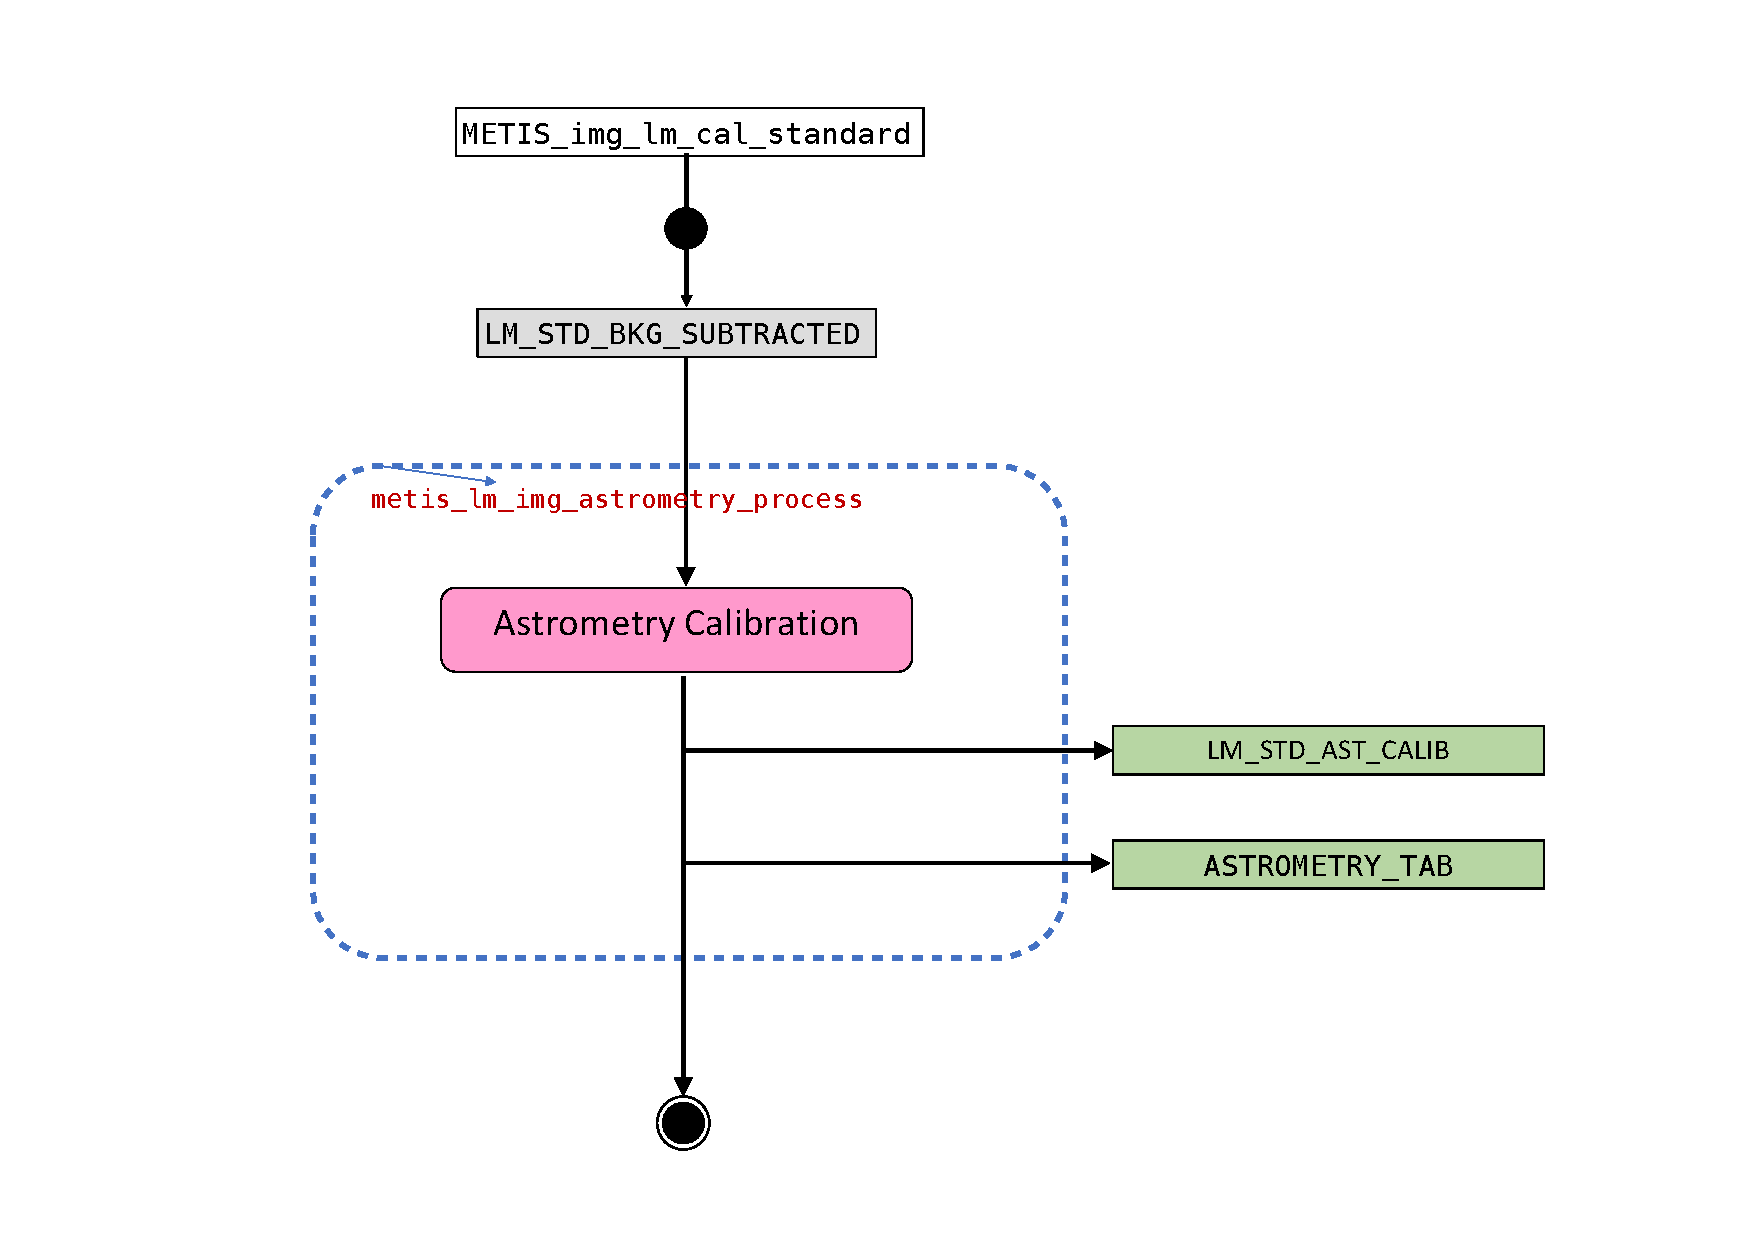
\includegraphics[width=1.0\textwidth]{metis_lm_img_astrometry_process}
%   %\resizebox{0.6\textwidth}{0.1\textwidth}{\TODO{\fbox{Figure to be done}}}
%   \caption[Recipe: \CODE{metis_lm_img_astrometry_process}]{\CODE{metis_lm_img_astrometry_process} --
%     compute conversion between pixel and sky coordinate}
%   \label{fig:metis_lm_img_astrometry_process}
% \end{figure}
%
%
% \clearpage

\subsubsection{\REC*{metis_lm_img_std_process}:  Photometric standard analysis}
\label{lm_img_photstd}
\label{rec:lm_img_photstd}
\label{sssec:lm_img_photstd}
\label{rec:metis_lm_img_std_process}

This recipe determines the conversion from ADU to physical units from
a set of reduced exposures of a photometric standard star. The flux of
the star is measured in each exposure in ADU, normalised to an
exposure time of 1~second and averaged over all exposures. In
addition, the exposures are stacked (after recentering on the standard
star, but without derotation) and the flux is measured in the combined
image. Comparison to the tabulated brightness of the star in the
observing filter yields the conversion factor from
$\mathrm{ADU\,s^{-1}}$ to $\mathrm{photons\,\,s^{-1}\,cm^{-2}}$.

QC parameter will include estimates of the sensitivity for the
detection of point sources and surface brightness sensitivity
following~\cite{visir_manual}.

\begin{recipedef}
  Name:                & \REC{metis_lm_img_std_process} \\
  Purpose:             & Determine the conversion factor between detector counts and physical source flux \\
%  Requirements:        & \REQ{METIS-XXXX} \\
%  Type:                & Calibration | Science | Technical \\
%  Templates:           & \TPL{...} \\
  Primary input:       & \PROD{LM_STD_BKG_SUBTRACTED} (N$\times$) \\
  Secondary inputs:    & \EXTCALIB{FLUXSTD_CATALOG} \\
  Matched keywords:    & \FITS{DRS.FILTER} \\
  Parameters:          & \CODE{metis_lm_img_std_process.stacking.method}\newline Name of the method used to combine the input images (\texttt{add}, \texttt{average}, \texttt{median}, \texttt{sigclip}), default \texttt{average} \\
  Algorithm:           & Call metis\_lm\_calculate\_std\_flux to measure flux in input images \\
                       & call hdrl\_resample\_compute to recenter the images \\
                       & call hdrl\_imagelist\_collapse to stack the images \\
                       & call metis\_lm\_calculate\_std\_flux on the stacked image to get flux of the star in detector units \\
                       & call metis\_calculate\_std\_fluxcal to calculate the conversion factor to physical units \\
                       & call metis\_calculate\_detection\_limits to compute background noise (std, rms) and compute detection limits \\
  Output data:         & \PROD{FLUXCAL_TAB} \\
                       & \PROD{LM_STD_COMBINED} \\
%  Expected accuracies: & \\
  QC1 parameters:      & \QC{QC LM STD AIRMASS} \\
                       & \QC{QC LM STD APERTURE CNTS} \\
                       & \QC{QC LM AREA SENS} \\
                       & \QC{QC LM IMG STD BACKGD RMS} \\
                       & \QC{QC LM STD ELLIP} \\
                       & \QC{QC LM STD FLUXCONV} \\
                       & \QC{QC LM STD FWHM} \\
                       & \QC{QC LM STD PEAK CNTS} \\
                       & \QC{QC LM SENS} \\
                       & \QC{QC LM STD STREHL} \\
\end{recipedef}



\begin{figure}[hb]
    \centering
    \def \globalscale {0.700000}
    \fontsize{10}{12}\selectfont
    %% Flowchart of metis_lm_img_std_process, generated by metisp/drld/generate_drld.py -- do not edit

% ADDING NEW DEFINITIONS -------------------------------------------- start
\definecolor{listingbg}{gray}{0.95}
\definecolor{darkgreen}{rgb}{0.0, 0.7, 0.0}
\definecolor{darkblue} {rgb}{0.0, 0.0, 0.7}
\definecolor{cyan} {rgb}{0.0, 0.4, 0.4}
\definecolor{darkred}  {rgb}{0.7, 0.0, 0.0}
\definecolor{darkorange}{rgb}{1.0, 0.49, 0.0}
\definecolor{violet}{rgb}{255, 0, 255}
\definecolor{turq}{rgb}{0.0, 0.7, 0.8}
\definecolor{fits}{rgb}{0.4, 0.1, 1}


\makeatletter
\lstdefinestyle{RAWstyle}{%
  basicstyle=\ttfamily\color{black}%
  \lst@ifdisplaystyle\scriptsize\fi}

\lstdefinestyle{PARstyle}{%
  basicstyle=\ttfamily\color{black}%
  \lst@ifdisplaystyle\scriptsize\fi}

\lstdefinestyle{DRLstyle}{%
  basicstyle=\ttfamily\color{black}%
  \lst@ifdisplaystyle\scriptsize\fi}

\lstdefinestyle{RECstyle}{%
  basicstyle=\ttfamily\color{black}%
  \lst@ifdisplaystyle\scriptsize\fi}

\lstdefinestyle{QCstyle}{%
  basicstyle=\ttfamily\color{black}%
  \lst@ifdisplaystyle\scriptsize\fi}

\lstdefinestyle{TPLstyle}{%
  basicstyle=\ttfamily\color{black}%
  \lst@ifdisplaystyle\scriptsize\fi}

\lstdefinestyle{PRODstyle}{%
  basicstyle=\ttfamily\color{black}%
  \lst@ifdisplaystyle\scriptsize\fi}

\lstdefinestyle{EXTCALIBstyle}{%
  basicstyle=\ttfamily\color{black}%
  \lst@ifdisplaystyle\scriptsize\fi}

\lstdefinestyle{STATCALIBstyle}{%
  basicstyle=\ttfamily\color{black}%
  \lst@ifdisplaystyle\scriptsize\fi}

\lstdefinestyle{FITSstyle}{%
  basicstyle=\ttfamily\color{black}%
  \lst@ifdisplaystyle\scriptsize\fi}
\makeatother

\input{recipe_config}
%% The picture is set in a box and only scaled down when it would not fit the page.
\ifdefined\flowchartbox\else\newsavebox{\flowchartbox}\fi
\sbox{\flowchartbox}{%
\begin{tikzpicture}
  [x=1cm,
  y=-1cm,
  align=center,
  node distance=2cm and 3.5cm,
  redstep/.append style={minimum height=0.8cm, text width=3.8cm}]
  \sffamily
  \pic (start){start};
  \node (input) [below=0.75cm of start-m, input] {%
    \textsl{N} \PROD{LM_STD_BKG_SUBTRACTED}};

  %% algorithm steps
  \node (step_detectstandardstarinindi) [below=1.6cm of input, redstep]{%
    Detect standard star in individual frames};
  \node (step_shiftandcombineimagesbas) [below=0.6cm of step_detectstandardstarinindi, redstep]{%
    shift and combine images based on the position of the standard star};
  \node (step_measurefluxfromstarinins) [below=1.25cm of step_shiftandcombineimagesbas, redstep]{%
    measure flux from star in instrumental units in combined image};
  \node (step_computeconversionfactort) [below=0.6cm of step_measurefluxfromstarinins, redstep]{%
    compute conversion factor to physical units};
  \node (step_measurebackgroundnoisean) [below=1.25cm of step_computeconversionfactort, redstep]{%
    measure background noise and calculate detection limits};
  \pic (stop) [below=0.9cm of step_measurebackgroundnoisean] {stop};

  \draw [connection_arrow] (start-m) -- (input);
  \draw [connection_arrow] (input) -- (step_detectstandardstarinindi);
  \draw [connection_arrow] (step_detectstandardstarinindi) -- (step_shiftandcombineimagesbas);
  \draw [connection_arrow] (step_shiftandcombineimagesbas) -- (step_measurefluxfromstarinins);
  \draw [connection_arrow] (step_measurefluxfromstarinins) -- (step_computeconversionfactort);
  \draw [connection_arrow] (step_computeconversionfactort) -- (step_measurebackgroundnoisean);
  \draw [connection_arrow] (step_measurebackgroundnoisean) -- (stop-t);

  %% calibration inputs, attached above the step that consumes them
  \node (connect_fluxstdcatalog) [connection] at ($(input.south) + (0, 0.97)$) {};
  \node (fluxstdcatalog) [left=of connect_fluxstdcatalog, external] {\EXTCALIB{FLUXSTD_CATALOG}};
  \draw [connection_arrow] (fluxstdcatalog) -- (connect_fluxstdcatalog);

  %% products, attached below the step that produces them
  \node (connect_imgstdcombined) [connection] at ($(step_shiftandcombineimagesbas.south) + (0, 0.62)$) {};
  \node (imgstdcombined) [right=of connect_imgstdcombined, sciproduct] {\PROD{LM_STD_COMBINED}};
  \draw [connection_arrow] (connect_imgstdcombined) -- (imgstdcombined);
  \node (connect_imgfluxcaltable) [connection] at ($(step_computeconversionfactort.south) + (0, 0.62)$) {};
  \node (imgfluxcaltable) [right=of connect_imgfluxcaltable, calproduct] {\PROD{FLUXCAL_TAB}};
  \draw [connection_arrow] (connect_imgfluxcaltable) -- (imgfluxcaltable);

  \draw [frame] ($(input.south) + (-2.85, 0.12)$) rectangle
  ($(step_measurebackgroundnoisean.south) + (2.85, 0.5)$);
  \node [framecolor, anchor=north west] at ($(input.south) + (-2.85, 0.12)$) {%
    \REC{metis_lm_img_std_process}};
\end{tikzpicture}}%
\ifdim\ht\flowchartbox>\dimexpr\textheight-4\baselineskip\relax
  \resizebox{!}{\dimexpr\textheight-4\baselineskip\relax}{\usebox{\flowchartbox}}%
\else\ifdim\wd\flowchartbox>\linewidth
  \resizebox{\linewidth}{!}{\usebox{\flowchartbox}}%
\else
  \usebox{\flowchartbox}%
\fi\fi

% ADDING NEW DEFINITIONS -------------------------------------------- start
\definecolor{listingbg}{gray}{0.95}
\definecolor{darkgreen}{rgb}{0.0, 0.7, 0.0}
\definecolor{darkblue} {rgb}{0.0, 0.0, 0.7}
\definecolor{cyan} {rgb}{0.0, 0.4, 0.4}
\definecolor{darkred}  {rgb}{0.7, 0.0, 0.0}
\definecolor{darkorange}{rgb}{1.0, 0.49, 0.0}
\definecolor{violet}{rgb}{255, 0, 255}
\definecolor{turq}{rgb}{0.0, 0.7, 0.8}
\definecolor{fits}{rgb}{0.4, 0.1, 1}


\makeatletter
\lstdefinestyle{RAWstyle}{%
  basicstyle=\ttfamily\color{fits}%
  \lst@ifdisplaystyle\scriptsize\fi}

\lstdefinestyle{PARstyle}{%
  basicstyle=\ttfamily\color{cyan}%
  \lst@ifdisplaystyle\scriptsize\fi}

\lstdefinestyle{DRLstyle}{%
  basicstyle=\ttfamily\color{violet}%
  \lst@ifdisplaystyle\scriptsize\fi}

\lstdefinestyle{RECstyle}{%
  basicstyle=\ttfamily\color{darkgreen}%
  \lst@ifdisplaystyle\scriptsize\fi}

%% Write QC parameters like this: \QC{QC_SOMETHING_OR_OTHER}
\lstdefinestyle{QCstyle}{%
  basicstyle=\ttfamily\color{darkblue}%
  \lst@ifdisplaystyle\scriptsize\fi}

%% Write templates like this: \TPL{DARK_LM}
\lstdefinestyle{TPLstyle}{%
  basicstyle=\ttfamily\color{darkred}%
  \lst@ifdisplaystyle\scriptsize\fi}

%% Write products like this: \PROD{SOME_THING}
\lstdefinestyle{PRODstyle}{%
  basicstyle=\ttfamily\color{darkorange}%
  \lst@ifdisplaystyle\scriptsize\fi}

%% external calib files
\lstdefinestyle{EXTCALIBstyle}{%
  basicstyle=\ttfamily\color{Turquoise}%
  \lst@ifdisplaystyle\scriptsize\fi}

% static calib files
\lstdefinestyle{STATCALIBstyle}{%
  basicstyle=\ttfamily\color{teal}%
  \lst@ifdisplaystyle\scriptsize\fi}

% static calib files
\lstdefinestyle{FITSstyle}{%
  basicstyle=\ttfamily\color{black}%
  \lst@ifdisplaystyle\scriptsize\fi}
\makeatother


  \caption[Recipe: \REC*{metis_lm_img_std_process}]{\REC*{metis_lm_img_std_process} --
    compute conversion between ADU and physical flux units}
  \label{fig:metis_lm_img_std_process}
\end{figure}

%%%%%%%%%%%%%%%%%%%%%%%%%%%%%%%%%%%%%%%%%%%%%%%%%
%------------------------------------------------------------------------------------------------------------------
\clearpage
\subsubsection{\REC*{metis_lm_img_calibrate}:  Image calibration}
\label{lm_img_calibrate}
\label{rec:metis_lm_img_calibrate}
\label{rec:lm_img_calibrate}
\label{sssec:lm_img_calibrate}

This recipe applies the flux calibration to the reduced science
images and adds geometric calibration data to the FITS header. The
products of this recipe are fully calibrated individual exposures.

Each image is multiplied by the conversion factor such that pixel
values are in units of photons per second per centimetre squared. The
header of each file receives keyword \FITS*{BUNIT} with value %
\CODE{'photon.s**(-1).cm**(-2)'}.

% Moved to https://github.com/AstarVienna/METIS_DRLD/issues/98
% \TODO{Other units may be possible, although additional information is
%   needed. For instance,\\ \CODE{photon.s**(-1).cm**(-2).arcsec**(-2)} makes
%   values independent of the pixel scale, but requires a distortion map
%   (variation of pixel scale across the detector). Energy units (erg
%   instead of photons) require knowledge of the spectral energy
%   distribution of the sources, in particular for broad-band filters.}

LM-band imaging observations will be performed in pupil-tracking mode
\cite{METIS-operational_concept}, which means that the field rotates
from exposure to exposure.  The information about the field
orientation along with target coordinates, pixel scale and
higher-order polynomial distortion coefficients is written to the FITS
header. The images are not resampled by this recipe, this is left to
 \REC{metis_lm_img_sci_postprocess}.



\begin{recipedef}
  Name:                & \REC{metis_lm_img_calibrate} \\
  Purpose:             & Determine optical distortion coefficients for the LM imager. \\
%  Requirements:        & \REQ{METIS-XXXX} \\
%  Type:                & Calibration | Science | Technical \\
%  Templates:           & \TPL{...} \\
  Primary input:       & \PROD{LM_SCI_BKG_SUBTRACTED} \\
  Secondary inputs:    & \PROD{FLUXCAL_TAB} \\
                       & \PROD{LM_DISTORTION_TABLE} \\
  Matched keywords:    & \FITS{DRS.FILTER} \\
  Parameters:          & \CODE{metis_lm_img_calibrate.stacking.method}: string\newline Name of the method used to combine the input images (\texttt{add}, \underline{\texttt{average}}, \texttt{median}, \texttt{sigclip}) \\
  Algorithm:           & Call metis\_lm\_scale\_image\_flux to scale image data to photon / s \\
                       & Add header information (BUNIT, WCS, etc.) \\
  Output data:         & \PROD{LM_SCI_CALIBRATED} \\
%  Expected accuracies: & \\
  QC1 parameters:      & --- none --- \\
\end{recipedef}



\begin{figure}[hb]
  \centering
  \def \globalscale {0.700000}
  \fontsize{10}{12}\selectfont
  %% Flowchart of metis_lm_img_calibrate, generated by metisp/drld/generate_drld.py -- do not edit

% ADDING NEW DEFINITIONS -------------------------------------------- start
\definecolor{listingbg}{gray}{0.95}
\definecolor{darkgreen}{rgb}{0.0, 0.7, 0.0}
\definecolor{darkblue} {rgb}{0.0, 0.0, 0.7}
\definecolor{cyan} {rgb}{0.0, 0.4, 0.4}
\definecolor{darkred}  {rgb}{0.7, 0.0, 0.0}
\definecolor{darkorange}{rgb}{1.0, 0.49, 0.0}
\definecolor{violet}{rgb}{255, 0, 255}
\definecolor{turq}{rgb}{0.0, 0.7, 0.8}
\definecolor{fits}{rgb}{0.4, 0.1, 1}


\makeatletter
\lstdefinestyle{RAWstyle}{%
  basicstyle=\ttfamily\color{black}%
  \lst@ifdisplaystyle\scriptsize\fi}

\lstdefinestyle{PARstyle}{%
  basicstyle=\ttfamily\color{black}%
  \lst@ifdisplaystyle\scriptsize\fi}

\lstdefinestyle{DRLstyle}{%
  basicstyle=\ttfamily\color{black}%
  \lst@ifdisplaystyle\scriptsize\fi}

\lstdefinestyle{RECstyle}{%
  basicstyle=\ttfamily\color{black}%
  \lst@ifdisplaystyle\scriptsize\fi}

\lstdefinestyle{QCstyle}{%
  basicstyle=\ttfamily\color{black}%
  \lst@ifdisplaystyle\scriptsize\fi}

\lstdefinestyle{TPLstyle}{%
  basicstyle=\ttfamily\color{black}%
  \lst@ifdisplaystyle\scriptsize\fi}

\lstdefinestyle{PRODstyle}{%
  basicstyle=\ttfamily\color{black}%
  \lst@ifdisplaystyle\scriptsize\fi}

\lstdefinestyle{EXTCALIBstyle}{%
  basicstyle=\ttfamily\color{black}%
  \lst@ifdisplaystyle\scriptsize\fi}

\lstdefinestyle{STATCALIBstyle}{%
  basicstyle=\ttfamily\color{black}%
  \lst@ifdisplaystyle\scriptsize\fi}

\lstdefinestyle{FITSstyle}{%
  basicstyle=\ttfamily\color{black}%
  \lst@ifdisplaystyle\scriptsize\fi}
\makeatother

\input{recipe_config}
%% The picture is set in a box and only scaled down when it would not fit the page.
\ifdefined\flowchartbox\else\newsavebox{\flowchartbox}\fi
\sbox{\flowchartbox}{%
\begin{tikzpicture}
  [x=1cm,
  y=-1cm,
  align=center,
  node distance=2cm and 3.5cm,
  redstep/.append style={minimum height=0.8cm, text width=3.8cm}]
  \sffamily
  \pic (start){start};
  \node (input) [below=0.75cm of start-m, input] {%
    \PROD{LM_SCI_BKG_SUBTRACTED}};

  %% algorithm steps
  \node (step_scaleimagedatatophotonss) [below=1.6cm of input, redstep]{%
    Scale image data to photons/s};
  \node (step_addbunitanddistortioninf) [below=1.25cm of step_scaleimagedatatophotonss, redstep]{%
    Add BUNIT and distortion information to header};
  \pic (stop) [below=1.45cm of step_addbunitanddistortioninf] {stop};

  \draw [connection_arrow] (start-m) -- (input);
  \draw [connection_arrow] (input) -- (step_scaleimagedatatophotonss);
  \draw [connection_arrow] (step_scaleimagedatatophotonss) -- (step_addbunitanddistortioninf);
  \draw [connection_arrow] (step_addbunitanddistortioninf) -- (stop-t);

  %% calibration inputs, attached above the step that consumes them
  \node (connect_fluxcaltable) [connection] at ($(input.south) + (0, 0.97)$) {};
  \node (fluxcaltable) [left=of connect_fluxcaltable, calproduct] {\PROD{FLUXCAL_TAB}};
  \draw [connection_arrow] (fluxcaltable) -- (connect_fluxcaltable);
  \node (connect_distortiontable) [connection] at ($(step_scaleimagedatatophotonss.south) + (0, 0.62)$) {};
  \node (distortiontable) [left=of connect_distortiontable, calproduct] {\PROD{LM_DISTORTION_TABLE}};
  \draw [connection_arrow] (distortiontable) -- (connect_distortiontable);

  %% products, attached below the step that produces them
  \node (connect_scicalibrated) [connection] at ($(step_addbunitanddistortioninf.south) + (0, 0.62)$) {};
  \node (scicalibrated) [right=of connect_scicalibrated, sciproduct] {\PROD{LM_SCI_CALIBRATED}};
  \draw [connection_arrow] (connect_scicalibrated) -- (scicalibrated);

  \draw [frame] ($(input.south) + (-2.85, 0.12)$) rectangle
  ($(step_addbunitanddistortioninf.south) + (2.85, 1.0499999999999998)$);
  \node [framecolor, anchor=north west] at ($(input.south) + (-2.85, 0.12)$) {%
    \REC{metis_lm_img_calibrate}};
\end{tikzpicture}}%
\ifdim\ht\flowchartbox>\dimexpr\textheight-4\baselineskip\relax
  \resizebox{!}{\dimexpr\textheight-4\baselineskip\relax}{\usebox{\flowchartbox}}%
\else\ifdim\wd\flowchartbox>\linewidth
  \resizebox{\linewidth}{!}{\usebox{\flowchartbox}}%
\else
  \usebox{\flowchartbox}%
\fi\fi

% ADDING NEW DEFINITIONS -------------------------------------------- start
\definecolor{listingbg}{gray}{0.95}
\definecolor{darkgreen}{rgb}{0.0, 0.7, 0.0}
\definecolor{darkblue} {rgb}{0.0, 0.0, 0.7}
\definecolor{cyan} {rgb}{0.0, 0.4, 0.4}
\definecolor{darkred}  {rgb}{0.7, 0.0, 0.0}
\definecolor{darkorange}{rgb}{1.0, 0.49, 0.0}
\definecolor{violet}{rgb}{255, 0, 255}
\definecolor{turq}{rgb}{0.0, 0.7, 0.8}
\definecolor{fits}{rgb}{0.4, 0.1, 1}


\makeatletter
\lstdefinestyle{RAWstyle}{%
  basicstyle=\ttfamily\color{fits}%
  \lst@ifdisplaystyle\scriptsize\fi}

\lstdefinestyle{PARstyle}{%
  basicstyle=\ttfamily\color{cyan}%
  \lst@ifdisplaystyle\scriptsize\fi}

\lstdefinestyle{DRLstyle}{%
  basicstyle=\ttfamily\color{violet}%
  \lst@ifdisplaystyle\scriptsize\fi}

\lstdefinestyle{RECstyle}{%
  basicstyle=\ttfamily\color{darkgreen}%
  \lst@ifdisplaystyle\scriptsize\fi}

%% Write QC parameters like this: \QC{QC_SOMETHING_OR_OTHER}
\lstdefinestyle{QCstyle}{%
  basicstyle=\ttfamily\color{darkblue}%
  \lst@ifdisplaystyle\scriptsize\fi}

%% Write templates like this: \TPL{DARK_LM}
\lstdefinestyle{TPLstyle}{%
  basicstyle=\ttfamily\color{darkred}%
  \lst@ifdisplaystyle\scriptsize\fi}

%% Write products like this: \PROD{SOME_THING}
\lstdefinestyle{PRODstyle}{%
  basicstyle=\ttfamily\color{darkorange}%
  \lst@ifdisplaystyle\scriptsize\fi}

%% external calib files
\lstdefinestyle{EXTCALIBstyle}{%
  basicstyle=\ttfamily\color{Turquoise}%
  \lst@ifdisplaystyle\scriptsize\fi}

% static calib files
\lstdefinestyle{STATCALIBstyle}{%
  basicstyle=\ttfamily\color{teal}%
  \lst@ifdisplaystyle\scriptsize\fi}

% static calib files
\lstdefinestyle{FITSstyle}{%
  basicstyle=\ttfamily\color{black}%
  \lst@ifdisplaystyle\scriptsize\fi}
\makeatother


  \caption[Recipe: \REC*{metis_lm_img_calibrate}]{\REC*{metis_lm_img_calibrate} --
    Convert images to physical flux units and update FITS header}
  \label{fig:metis_lm_img_calibrate}
\end{figure}


%%%%%%%%%%%%%%%%%%%%%%%%%%%%
%------------------------------------------------------------------------------------------------------------------
\clearpage
\subsubsection{\REC*{metis_lm_img_sci_postprocess}:  Image post-processing}
\label{lm_img_postprocess}
\label{rec:lm_img_postprocess}
\label{sssec:lm_img_postprocess}
\label{rec:metis_lm_img_sci_postprocess}

This recipe coadds a sequence of flux-calibrated,
background-subtracted images (possibly from several observing blocks)
after resampling the images on a common pixel grid defined by a
standard sky projection.
% The alignment of the images (\FITS{CRVAL} keywords, rotation) may have to be checked and refined through cross-correlation of the overlapping images (TBC).
The alignment of the images is done through by using the position of the \ac{WFS-FS} mirror.
% TODO: Decide how the WFS-FS data is stored in the raw data.
% See https://github.com/AstarVienna/METIS_DRLD/issues/162
The number of input
images contributing to any pixel in the output image (variable due to
offsets and bad pixels) will be documented in a contribution
map.

The output files fulfill the \ac{SDP} criteria and are compliant with \REQ{METIS-6104}.

\begin{recipedef}
  Name:                & \REC{metis_lm_img_sci_postprocess} \\
  Purpose:             & Coadd reduced images \\
%  Requirements:        & \REQ{METIS-XXXX} \\
%  Type:                & Calibration | Science | Technical \\
%  Templates:           & \TPL{...} \\
  Primary input:       & \PROD{LM_SCI_CALIBRATED} (N$\times$) \\
  Secondary inputs:    & --- none --- \\
  Matched keywords:    & \FITS{DRS.FILTER} \\
  Parameters:          & \CODE{metis_lm_img_sci_postprocess.stacking.method}: string\newline Name of the method used to combine the input images (\texttt{add}, \underline{\texttt{average}}, \texttt{median}, \texttt{sigclip}) \\
  Algorithm:           & Check and refine WCS of input images by using the WFS-FS data. \\
                       & Determine output pixel grid encompassing all input images. \\
                       & Call hdrl\_resample\_compute to recenter the images. \\
                       & Call hdrl\_imagelist\_collapse to stack the images. \\
  Output data:         & \PROD{LM_SCI_COADD} \\
%  Expected accuracies: & \\
  QC1 parameters:      & \QC{QC LM SCI POSTPROC DELTAC} \\
                       & \QC{QC LM SCI POSTPROC GRIDRNG} \\
                       & \QC{QC LM SCI POSTPROC MEDMEAN} \\
                       & \QC{QC LM SCI POSTPROC MEDMED} \\
                       & \QC{QC LM SCI POSTPROC MEDRMS} \\
                       & \QC{QC LM SCI NEXP} \\
\end{recipedef}



\begin{figure}[hb]
    \centering
    \def \globalscale {0.700000}
    \fontsize{10}{12}\selectfont
    %% Flowchart of metis_lm_img_sci_postprocess, generated by metisp/drld/generate_drld.py -- do not edit

% ADDING NEW DEFINITIONS -------------------------------------------- start
\definecolor{listingbg}{gray}{0.95}
\definecolor{darkgreen}{rgb}{0.0, 0.7, 0.0}
\definecolor{darkblue} {rgb}{0.0, 0.0, 0.7}
\definecolor{cyan} {rgb}{0.0, 0.4, 0.4}
\definecolor{darkred}  {rgb}{0.7, 0.0, 0.0}
\definecolor{darkorange}{rgb}{1.0, 0.49, 0.0}
\definecolor{violet}{rgb}{255, 0, 255}
\definecolor{turq}{rgb}{0.0, 0.7, 0.8}
\definecolor{fits}{rgb}{0.4, 0.1, 1}


\makeatletter
\lstdefinestyle{RAWstyle}{%
  basicstyle=\ttfamily\color{black}%
  \lst@ifdisplaystyle\scriptsize\fi}

\lstdefinestyle{PARstyle}{%
  basicstyle=\ttfamily\color{black}%
  \lst@ifdisplaystyle\scriptsize\fi}

\lstdefinestyle{DRLstyle}{%
  basicstyle=\ttfamily\color{black}%
  \lst@ifdisplaystyle\scriptsize\fi}

\lstdefinestyle{RECstyle}{%
  basicstyle=\ttfamily\color{black}%
  \lst@ifdisplaystyle\scriptsize\fi}

\lstdefinestyle{QCstyle}{%
  basicstyle=\ttfamily\color{black}%
  \lst@ifdisplaystyle\scriptsize\fi}

\lstdefinestyle{TPLstyle}{%
  basicstyle=\ttfamily\color{black}%
  \lst@ifdisplaystyle\scriptsize\fi}

\lstdefinestyle{PRODstyle}{%
  basicstyle=\ttfamily\color{black}%
  \lst@ifdisplaystyle\scriptsize\fi}

\lstdefinestyle{EXTCALIBstyle}{%
  basicstyle=\ttfamily\color{black}%
  \lst@ifdisplaystyle\scriptsize\fi}

\lstdefinestyle{STATCALIBstyle}{%
  basicstyle=\ttfamily\color{black}%
  \lst@ifdisplaystyle\scriptsize\fi}

\lstdefinestyle{FITSstyle}{%
  basicstyle=\ttfamily\color{black}%
  \lst@ifdisplaystyle\scriptsize\fi}
\makeatother

\input{recipe_config}
%% The picture is set in a box and only scaled down when it would not fit the page.
\ifdefined\flowchartbox\else\newsavebox{\flowchartbox}\fi
\sbox{\flowchartbox}{%
\begin{tikzpicture}
  [x=1cm,
  y=-1cm,
  align=center,
  node distance=2cm and 3.5cm,
  redstep/.append style={minimum height=0.8cm, text width=3.8cm}]
  \sffamily
  \pic (start){start};
  \node (input) [below=0.75cm of start-m, input] {%
    \textsl{N} \PROD{LM_SCI_CALIBRATED}};

  %% algorithm steps
  \node (step_determineoutputgrid) [below=0.6cm of input, redstep]{%
    determine output grid};
  \node (step_resampleimages) [below=0.6cm of step_determineoutputgrid, redstep]{%
    resample images};
  \node (step_coaddimages) [below=0.6cm of step_resampleimages, redstep]{%
    coadd images};
  \pic (stop) [below=1.45cm of step_coaddimages] {stop};

  \draw [connection_arrow] (start-m) -- (input);
  \draw [connection_arrow] (input) -- (step_determineoutputgrid);
  \draw [connection_arrow] (step_determineoutputgrid) -- (step_resampleimages);
  \draw [connection_arrow] (step_resampleimages) -- (step_coaddimages);
  \draw [connection_arrow] (step_coaddimages) -- (stop-t);

  %% calibration inputs, attached above the step that consumes them

  %% products, attached below the step that produces them
  \node (connect_lmimgscicoadd) [connection] at ($(step_coaddimages.south) + (0, 0.62)$) {};
  \node (lmimgscicoadd) [right=of connect_lmimgscicoadd, sciproduct] {\PROD{LM_SCI_COADD}};
  \draw [connection_arrow] (connect_lmimgscicoadd) -- (lmimgscicoadd);

  \draw [frame] ($(input.south) + (-2.85, 0.12)$) rectangle
  ($(step_coaddimages.south) + (2.85, 1.0499999999999998)$);
  \node [framecolor, anchor=north west] at ($(input.south) + (-2.85, 0.12)$) {%
    \REC{metis_lm_img_sci_postprocess}};
\end{tikzpicture}}%
\ifdim\ht\flowchartbox>\dimexpr\textheight-4\baselineskip\relax
  \resizebox{!}{\dimexpr\textheight-4\baselineskip\relax}{\usebox{\flowchartbox}}%
\else\ifdim\wd\flowchartbox>\linewidth
  \resizebox{\linewidth}{!}{\usebox{\flowchartbox}}%
\else
  \usebox{\flowchartbox}%
\fi\fi

% ADDING NEW DEFINITIONS -------------------------------------------- start
\definecolor{listingbg}{gray}{0.95}
\definecolor{darkgreen}{rgb}{0.0, 0.7, 0.0}
\definecolor{darkblue} {rgb}{0.0, 0.0, 0.7}
\definecolor{cyan} {rgb}{0.0, 0.4, 0.4}
\definecolor{darkred}  {rgb}{0.7, 0.0, 0.0}
\definecolor{darkorange}{rgb}{1.0, 0.49, 0.0}
\definecolor{violet}{rgb}{255, 0, 255}
\definecolor{turq}{rgb}{0.0, 0.7, 0.8}
\definecolor{fits}{rgb}{0.4, 0.1, 1}


\makeatletter
\lstdefinestyle{RAWstyle}{%
  basicstyle=\ttfamily\color{fits}%
  \lst@ifdisplaystyle\scriptsize\fi}

\lstdefinestyle{PARstyle}{%
  basicstyle=\ttfamily\color{cyan}%
  \lst@ifdisplaystyle\scriptsize\fi}

\lstdefinestyle{DRLstyle}{%
  basicstyle=\ttfamily\color{violet}%
  \lst@ifdisplaystyle\scriptsize\fi}

\lstdefinestyle{RECstyle}{%
  basicstyle=\ttfamily\color{darkgreen}%
  \lst@ifdisplaystyle\scriptsize\fi}

%% Write QC parameters like this: \QC{QC_SOMETHING_OR_OTHER}
\lstdefinestyle{QCstyle}{%
  basicstyle=\ttfamily\color{darkblue}%
  \lst@ifdisplaystyle\scriptsize\fi}

%% Write templates like this: \TPL{DARK_LM}
\lstdefinestyle{TPLstyle}{%
  basicstyle=\ttfamily\color{darkred}%
  \lst@ifdisplaystyle\scriptsize\fi}

%% Write products like this: \PROD{SOME_THING}
\lstdefinestyle{PRODstyle}{%
  basicstyle=\ttfamily\color{darkorange}%
  \lst@ifdisplaystyle\scriptsize\fi}

%% external calib files
\lstdefinestyle{EXTCALIBstyle}{%
  basicstyle=\ttfamily\color{Turquoise}%
  \lst@ifdisplaystyle\scriptsize\fi}

% static calib files
\lstdefinestyle{STATCALIBstyle}{%
  basicstyle=\ttfamily\color{teal}%
  \lst@ifdisplaystyle\scriptsize\fi}

% static calib files
\lstdefinestyle{FITSstyle}{%
  basicstyle=\ttfamily\color{black}%
  \lst@ifdisplaystyle\scriptsize\fi}
\makeatother


  \caption[Recipe: \REC*{metis_lm_img_sci_postprocess}]{%
    \REC{metis_lm_img_sci_postprocess} -- post-processing (coaddition)
    of reduced \CODE{IMG_LM} science frames.}
  \label{fig:metis_lm_img_sci_postprocess}
\end{figure}

%%%%%%%%%%%%%%%%%%%%%%%%%%%%%%%%%%%%%%%%%%%%
%------------------------------------------------------------------------------------------------------------------
\clearpage
\subsubsection{\REC*{metis_lm_img_distortion}:  Distortion calibration}
\label{rec:metis_lm_img_distortion}
\label{lm_img_distortion}
\label{rec:lm_img_distortion}
\label{sssec:lm_img_distortion}

Calibration of the imaging distortion is done on an image of a
pin-hole grid mask located in the \ac{WCU}. The
distortion is described in terms of a polynomial model whose
coefficients can be transformed to WCS keywords and applied to any
other pipeline product. In addition to the distortion table, a map of
pixel scale across the detector will be created.

\begin{recipedef}
  Name:                & \REC{metis_lm_img_distortion} \\
  Purpose:             & Determine optical distortion coefficients for the LM imager. \\
%  Requirements:        & \REQ{METIS-XXXX} \\
%  Type:                & Calibration | Science | Technical \\
%  Templates:           & \TPL{...} \\
  Primary input:       & \RAW{LM_DISTORTION_RAW} (N$\times$) \\
                       & \RAW{LM_WCU_OFF_RAW} (N$\times$) \\
  Secondary inputs:    & \PROD{BADPIX_MAP_2RG} (optional) \\
                       & \hyperref[dataitem:gain_map_det]{\STATCALIB*{GAIN_MAP_2RG}} \\
                       & \hyperref[dataitem:linearity_det]{\PROD*{LINEARITY_2RG}} \\
                       & \EXTCALIB{PERSISTENCE_MAP} (optional) \\
                       & \EXTCALIB{PINHOLE_TABLE} \\
  Matched keywords:    & \FITS{DRS.FILTER} \\
  Parameters:          & \CODE{metis_lm_img_distortion.stacking.method}\newline Name of the method used to combine the input images (\texttt{add}, \texttt{average}, \texttt{median}, \texttt{sigclip}), default \texttt{average} \\
  Algorithm:           & Subtract background image with \texttt{hdrl\_imagelist\_sub\_image}. \\
                       & Measure location of point source images in frames with \texttt{hdrl\_catalogue\_create}. \\
                       & Call metis\_fit\_distortion to fit polynomial coefficients to deviations from grid positions. \\
  Output data:         & \PROD{LM_DISTORTION_MAP} \\
                       & \PROD{LM_DIST_REDUCED} \\
                       & \PROD{LM_DISTORTION_TABLE} \\
%  Expected accuracies: & \\
  QC1 parameters:      & \QC{QC LM DISTORT NSOURCE} \\
                       & \QC{QC LM DISTORT RMS} \\
\end{recipedef}




\newgeometry{bottom=0.5cm, right=0.5cm, left=0.5cm}
\begin{figure}[hb]
    \centering
    \def \globalscale {0.700000}
    \fontsize{10}{12}\selectfont
    %% Flowchart of metis_lm_img_distortion, generated by metisp/drld/generate_drld.py -- do not edit

% ADDING NEW DEFINITIONS -------------------------------------------- start
\definecolor{listingbg}{gray}{0.95}
\definecolor{darkgreen}{rgb}{0.0, 0.7, 0.0}
\definecolor{darkblue} {rgb}{0.0, 0.0, 0.7}
\definecolor{cyan} {rgb}{0.0, 0.4, 0.4}
\definecolor{darkred}  {rgb}{0.7, 0.0, 0.0}
\definecolor{darkorange}{rgb}{1.0, 0.49, 0.0}
\definecolor{violet}{rgb}{255, 0, 255}
\definecolor{turq}{rgb}{0.0, 0.7, 0.8}
\definecolor{fits}{rgb}{0.4, 0.1, 1}


\makeatletter
\lstdefinestyle{RAWstyle}{%
  basicstyle=\ttfamily\color{black}%
  \lst@ifdisplaystyle\scriptsize\fi}

\lstdefinestyle{PARstyle}{%
  basicstyle=\ttfamily\color{black}%
  \lst@ifdisplaystyle\scriptsize\fi}

\lstdefinestyle{DRLstyle}{%
  basicstyle=\ttfamily\color{black}%
  \lst@ifdisplaystyle\scriptsize\fi}

\lstdefinestyle{RECstyle}{%
  basicstyle=\ttfamily\color{black}%
  \lst@ifdisplaystyle\scriptsize\fi}

\lstdefinestyle{QCstyle}{%
  basicstyle=\ttfamily\color{black}%
  \lst@ifdisplaystyle\scriptsize\fi}

\lstdefinestyle{TPLstyle}{%
  basicstyle=\ttfamily\color{black}%
  \lst@ifdisplaystyle\scriptsize\fi}

\lstdefinestyle{PRODstyle}{%
  basicstyle=\ttfamily\color{black}%
  \lst@ifdisplaystyle\scriptsize\fi}

\lstdefinestyle{EXTCALIBstyle}{%
  basicstyle=\ttfamily\color{black}%
  \lst@ifdisplaystyle\scriptsize\fi}

\lstdefinestyle{STATCALIBstyle}{%
  basicstyle=\ttfamily\color{black}%
  \lst@ifdisplaystyle\scriptsize\fi}

\lstdefinestyle{FITSstyle}{%
  basicstyle=\ttfamily\color{black}%
  \lst@ifdisplaystyle\scriptsize\fi}
\makeatother

\input{recipe_config}
%% The picture is set in a box and only scaled down when it would not fit the page.
\ifdefined\flowchartbox\else\newsavebox{\flowchartbox}\fi
\sbox{\flowchartbox}{%
\begin{tikzpicture}
  [x=1cm,
  y=-1cm,
  align=center,
  node distance=2cm and 3.5cm,
  redstep/.append style={minimum height=0.8cm, text width=3.8cm}]
  \sffamily
  \pic (start){start};
  \node (input) [below=0.75cm of start-m, input] {%
    N$\times$ \RAW{LM_DISTORTION_RAW} \\[-0.5ex] {\footnotesize or} \\[-0.5ex]
    N$\times$ \RAW{LM_WCU_OFF_RAW}};

  %% algorithm steps
  \node (step_detectorsignatureremoval) [below=4.6cm of input, redstep]{%
    detector signature removal};
  \node (step_subtractwcuoffdark) [below=0.6cm of step_detectorsignatureremoval, redstep]{%
    subtract WCU OFF dark};
  \node (step_locateimages) [below=1.25cm of step_subtractwcuoffdark, redstep]{%
    locate images};
  \node (step_fitpolynomial) [below=0.6cm of step_locateimages, redstep]{%
    fit polynomial};
  \pic (stop) [below=3.45cm of step_fitpolynomial] {stop};

  \draw [connection_arrow] (start-m) -- (input);
  \draw [connection_arrow] (input) -- (step_detectorsignatureremoval);
  \draw [connection_arrow] (step_detectorsignatureremoval) -- (step_subtractwcuoffdark);
  \draw [connection_arrow] (step_subtractwcuoffdark) -- (step_locateimages);
  \draw [connection_arrow] (step_locateimages) -- (step_fitpolynomial);
  \draw [connection_arrow] (step_fitpolynomial) -- (stop-t);

  %% calibration inputs, attached above the step that consumes them
  \node (connect_badpixmap) [connection] at ($(input.south) + (0, 0.97)$) {};
  \node (badpixmap) [left=of connect_badpixmap, calproduct] {\PROD{BADPIX_MAP_2RG}};
  \draw [connection_arrow, dashed] (badpixmap) -- (connect_badpixmap);
  \node (connect_gainmap) [connection] at ($(input.south) + (0, 1.98)$) {};
  \node (gainmap) [left=of connect_gainmap, external] {\hyperref[dataitem:gain_map_det]{\STATCALIB*{GAIN_MAP_2RG}}};
  \draw [connection_arrow] (gainmap) -- (connect_gainmap);
  \node (connect_linearity) [connection] at ($(input.south) + (0, 2.98)$) {};
  \node (linearity) [left=of connect_linearity, calproduct] {\hyperref[dataitem:linearity_det]{\PROD*{LINEARITY_2RG}}};
  \draw [connection_arrow] (linearity) -- (connect_linearity);
  \node (connect_persistencemap) [connection] at ($(input.south) + (0, 3.98)$) {};
  \node (persistencemap) [left=of connect_persistencemap, external] {\EXTCALIB{PERSISTENCE_MAP}};
  \draw [connection_arrow, dashed] (persistencemap) -- (connect_persistencemap);
  \node (connect_pinholetable) [connection] at ($(step_subtractwcuoffdark.south) + (0, 0.62)$) {};
  \node (pinholetable) [left=of connect_pinholetable, external] {\EXTCALIB{PINHOLE_TABLE}};
  \draw [connection_arrow] (pinholetable) -- (connect_pinholetable);

  %% products, attached below the step that produces them
  \node (connect_distortionmap) [connection] at ($(step_fitpolynomial.south) + (0, 0.62)$) {};
  \node (distortionmap) [right=of connect_distortionmap, calproduct] {\PROD{LM_DISTORTION_MAP}};
  \draw [connection_arrow] (connect_distortionmap) -- (distortionmap);
  \node (connect_distortionreduced) [connection] at ($(step_fitpolynomial.south) + (0, 1.62)$) {};
  \node (distortionreduced) [right=of connect_distortionreduced, calproduct] {\PROD{LM_DIST_REDUCED}};
  \draw [connection_arrow] (connect_distortionreduced) -- (distortionreduced);
  \node (connect_distortiontable) [connection] at ($(step_fitpolynomial.south) + (0, 2.62)$) {};
  \node (distortiontable) [right=of connect_distortiontable, calproduct] {\PROD{LM_DISTORTION_TABLE}};
  \draw [connection_arrow] (connect_distortiontable) -- (distortiontable);

  \draw [frame] ($(input.south) + (-2.85, 0.12)$) rectangle
  ($(step_fitpolynomial.south) + (2.85, 3.0500000000000003)$);
  \node [framecolor, anchor=north west] at ($(input.south) + (-2.85, 0.12)$) {%
    \REC{metis_lm_img_distortion}};
\end{tikzpicture}}%
\ifdim\ht\flowchartbox>\dimexpr\textheight-4\baselineskip\relax
  \resizebox{!}{\dimexpr\textheight-4\baselineskip\relax}{\usebox{\flowchartbox}}%
\else\ifdim\wd\flowchartbox>\linewidth
  \resizebox{\linewidth}{!}{\usebox{\flowchartbox}}%
\else
  \usebox{\flowchartbox}%
\fi\fi

% ADDING NEW DEFINITIONS -------------------------------------------- start
\definecolor{listingbg}{gray}{0.95}
\definecolor{darkgreen}{rgb}{0.0, 0.7, 0.0}
\definecolor{darkblue} {rgb}{0.0, 0.0, 0.7}
\definecolor{cyan} {rgb}{0.0, 0.4, 0.4}
\definecolor{darkred}  {rgb}{0.7, 0.0, 0.0}
\definecolor{darkorange}{rgb}{1.0, 0.49, 0.0}
\definecolor{violet}{rgb}{255, 0, 255}
\definecolor{turq}{rgb}{0.0, 0.7, 0.8}
\definecolor{fits}{rgb}{0.4, 0.1, 1}


\makeatletter
\lstdefinestyle{RAWstyle}{%
  basicstyle=\ttfamily\color{fits}%
  \lst@ifdisplaystyle\scriptsize\fi}

\lstdefinestyle{PARstyle}{%
  basicstyle=\ttfamily\color{cyan}%
  \lst@ifdisplaystyle\scriptsize\fi}

\lstdefinestyle{DRLstyle}{%
  basicstyle=\ttfamily\color{violet}%
  \lst@ifdisplaystyle\scriptsize\fi}

\lstdefinestyle{RECstyle}{%
  basicstyle=\ttfamily\color{darkgreen}%
  \lst@ifdisplaystyle\scriptsize\fi}

%% Write QC parameters like this: \QC{QC_SOMETHING_OR_OTHER}
\lstdefinestyle{QCstyle}{%
  basicstyle=\ttfamily\color{darkblue}%
  \lst@ifdisplaystyle\scriptsize\fi}

%% Write templates like this: \TPL{DARK_LM}
\lstdefinestyle{TPLstyle}{%
  basicstyle=\ttfamily\color{darkred}%
  \lst@ifdisplaystyle\scriptsize\fi}

%% Write products like this: \PROD{SOME_THING}
\lstdefinestyle{PRODstyle}{%
  basicstyle=\ttfamily\color{darkorange}%
  \lst@ifdisplaystyle\scriptsize\fi}

%% external calib files
\lstdefinestyle{EXTCALIBstyle}{%
  basicstyle=\ttfamily\color{Turquoise}%
  \lst@ifdisplaystyle\scriptsize\fi}

% static calib files
\lstdefinestyle{STATCALIBstyle}{%
  basicstyle=\ttfamily\color{teal}%
  \lst@ifdisplaystyle\scriptsize\fi}

% static calib files
\lstdefinestyle{FITSstyle}{%
  basicstyle=\ttfamily\color{black}%
  \lst@ifdisplaystyle\scriptsize\fi}
\makeatother


    \caption[Recipe: \REC*{metis_lm_img_distortion}]{%
    \REC{metis_lm_img_distortion} -- LM IMG distortion calibration}
  \label{fig:metis_lm_img_distortion}
\end{figure}
\restoregeometry

\FloatBarrier

%%% Local Variables:
%%% TeX-master: "METIS_DRLD"
%%% End:
